\documentclass[12pt]{beamer}

\usepackage{algpseudocode}
\usepackage{graphicx}
\renewcommand{\algorithmicrequire}{\textbf{Input:}}
\renewcommand{\algorithmicensure}{\textbf{Output:}}

\author{Jake Humphrey}
\title{A Stochastic Computational Approach for Accurate and Efficient Reliability Evaluation}
\subtitle{A Python Implementation}
\institute{Department of Electronic and Electrical Engineering\\
  Imperial College London\\
  \texttt{jbh111@ic.ac.uk}
}

\begin{document}

\begin{frame}[plain]
  \titlepage
\end{frame}

\begin{frame}{Reliability of Circuits}
Gates in a logic circuit are, alas, not perfect. They are susceptible to error, of which there are three main types:
\begin{itemize}
\item \textbf{Stuck-At-One Error:} The output of the gate goes high, regardless of the expected output.
\item \textbf{Stuck-At-Zero Error:} The output of the gate goes low, regardless of the expected output.
\item \textbf{Von Neumann Error:} The output of the gate becomes the inverse of the expected output.
\end{itemize}
\end{frame}

\begin{frame}{Masking Effects}
However, there is a chance that errors in one gate will not propagate all the way to an output. This could be due to one of the following \emph{masking effect}s
\begin{itemize}
\item \textbf{Electrical Masking:} The error does not have a large enough effect on the amplitude of the logic signal to be detected at an input.
\item \textbf{Temporal Masking:} The error is input to a latch but occurs at some point in time outside of the latch's detection window.
\item \textbf{Logical Masking:} The error does not pass through a multi-input logic gate because the value of the other input(s) fix(es) the output of the gate.
\end{itemize}
\end{frame}
\begin{frame}{Reliability Analysis \small Principles}
As it happens, Logical Masking is the most prominent masking type in logical circuits. It is therefore useful to be able to analyse circuits on their ability to logically mask errors.
\vspace{0.25cm}

If we define the \emph{probability} of a signal as the proportion of time that it is logically True, then the basic idea is as follows:
\begin{itemize}
\item Construct a faulty representation of the circuit, which takes into account probabilities of each gate failing.
\item Derive the probabilities of the output signals.% in terms of the input probabilities and gate error probabilities for both the ideal and faulty circuits.
\item Then the \emph{reliability} of an output signal is the probability that it takes the same value in both the ideal and faulty circuits.
\end{itemize}
\end{frame}

\begin{frame}{Reliability Analysis \small Probabilistic Gate Models}
\only<1>{
However, existing algorithms are inefficient!
\vspace{0.25cm}

For example, \emph{Probabilistic Gate Models} (PGMs) attempt to analytically derive the output probabilities as functions of the input probabilities and gate error probabilities. 
}
\only<2>{
The problem occurs when the inputs to a gate are not statistically independent, such as is the case when there are \emph{reconvergent fanouts}. That is, when two or more inputs to a gate originated from a single signal.
\vspace{0.25cm}

The PGM equations do not account for statistically dependent signals, and the solution involves splitting the circuit into two sub-circuits. This approximately doubles the cost of the algorithm for each reconvergent fanout.
}
\end{frame}

\begin{frame}{Reliability Analysis \small Stochastic Logic}
The use of \emph{Stochastic Logic} can avoid these issues. With this approach, the input probabilities are used to generate input bitstreams, which are then propagated through the circuit. The output probabilities can then be accurately calculated from the output bitstreams.
\end{frame}

\begin{frame}{Reliability Analysis \small Stochastic Logic with Bernoulli Sequences}

Existing Stochastic Logic algorithms use the input probabilities to generate \emph{Bernoulli Sequences} of the form:

\begin{equation*}
[X_0, X_1 \dots X_{n-1}]; X_i \sim B(p)
\end{equation*}

for each input, where $p$ is the input probability.
\vspace{0.25cm}

However, this approach incurs a large computational overhead, as $n$ random numbers must be generated for each input. This can be significant for large circuits, because $n$ must be large to obtain accurate results.
\end{frame}

\begin{frame}{Reliability Analysis \small Stochastic Logic with Non-Bernoulli Sequences}
To reduce the random number generation overhead, \emph{Non-Bernoulli Sequences} can be used.
\vspace{0.25cm}

These sequences are generated deterministically with the expected number of 1s, and then randomly permuted.
\vspace{0.25cm}

This means only one random number generation is required per input bitstream.
\end{frame}

\begin{frame}{Reliability Analysis Algorithm}
The information on the previous slides gives rise to an algorithm for Reliability Analysis using Stochastic Logic with Non-Bernoulli Sequences.
\vspace{0.25cm}

I have written a Python implementation of this algorithm, which I will describe over the following slides.
\end{frame}

\begin{frame}[fragile]{Reliability Analysis Algorithm \small Pseudocode}
\only<1>{
\begin{algorithmic}
\Require Logic circuit to be tested
\Ensure Reliabilities for each output
\State $faulty\_circuit \gets  circuit $
\For{gate in circuit.gates}
	\State $faulty\_circuit.gates.add(error\_gate)$
	\State $faulty\_circuit.inputs.add(error\_signal)$
\EndFor
\For{input in faulty\_circuit.inputs}
	\State $input.stream \gets [False]\times SEQLEN$
	\State $input.stream[0:input.prob\times SEQLEN] \gets True$
	\State $shuffle(input.stream)$
\EndFor
\end{algorithmic}}

\only<2>{
\begin{algorithmic}
\For{output in circuit.outputs}
	\State $correct \gets []$
	\For{i from 0 to SEQLEN-1}
		\State $sigin \gets circuit.inputs[i]$
		\State $trueval \gets propagate(sigin, circuit, output)$
		\State $faultval \gets propagate(sigin, faulty\_circuit, output)$
		\State $correct.append(trueval == faultval)$
	\EndFor
	\State $output.reliability \gets correct.count(True)/SEQLEN$
\EndFor
\State \Return [output.reliability for output in circuit.outputs]
\end{algorithmic}}
\end{frame}

\begin{frame}{Reliability Analysis Algorithm \small Complexity Analysis}
The most costly section is the final double loop!
\vspace{0.25cm}

We have to propagate a signal through each circuit once for each output, and SEQLEN times.
\vspace{0.25cm}

The propagation could be at worst O(number of gates in the circuit), if the signal has to propagate through each gate.
\vspace{0.25cm}

If we let $o$ be the number of outputs of the circuit, $n$ be the length of the Non-Bernoulli Sequences, and $g$ be the number of gates in the circuit, we have that the complexity of the algorithm is $O(ogn)$
\end{frame}

\begin{frame}[fragile]{Reliability Analysis Algorithm \small Further Work}
This algorithm still has room for improvement. If \verb|propagate| is called once per output for the same input vector, it has to redundantly recalculate many intermediate values.
\vspace{0.25cm}

An improved \verb|propagate| would calculate all the output values in one go, thus reducing the double loop to a single one over the length of the input sequences.
\vspace{0.25cm}

This would reduce the algorithm complexity to $O(gn)$
\end{frame}

\begin{frame}{Reliability Analysis Algorithm \small Runtime Analysis}
\center
\only<1>{
\begin{tabular}{l|r r}
	Input Files & c17.v& c432.v\\
  \hline
  Inputs & 5 & 36\\
  Outputs & 2 & 7\\
  Gates & 6 & 160\\
  \hline
  Input Sequence Length & runtime /s & runtime /s\\
  \hline
  1 & 0.00023 & 1.34\\
  10 & 0.00067 & 12.2\\
  100 & 0.00485 & 122\\
  1 000 & 0.0473 & 1250\\
  10 000 & 0.458 & No Data\\
  100 000 & 4.66 & No Data
\end{tabular}}
\only<2>{
\begin{figure}
  \centering
    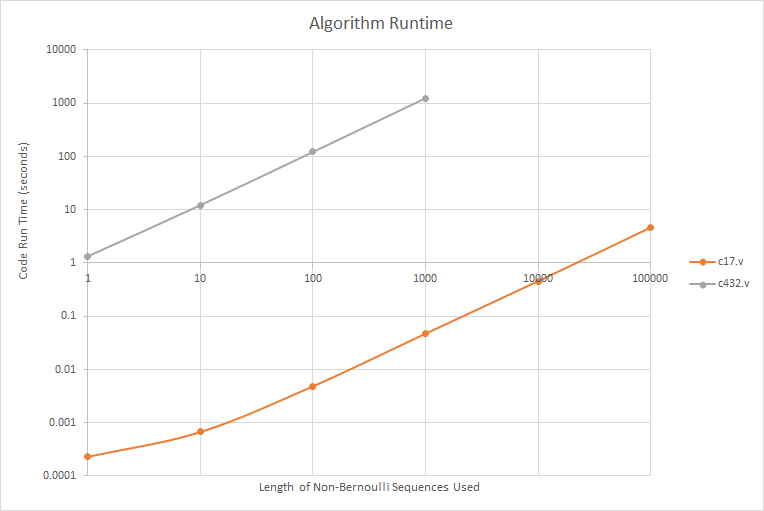
\includegraphics[width=\textwidth]{runtime}
\end{figure}
}
\end{frame}
\end{document}